\begin{figure*}[h]
\centering{
    \begin{tabular}{ccc}	
	
    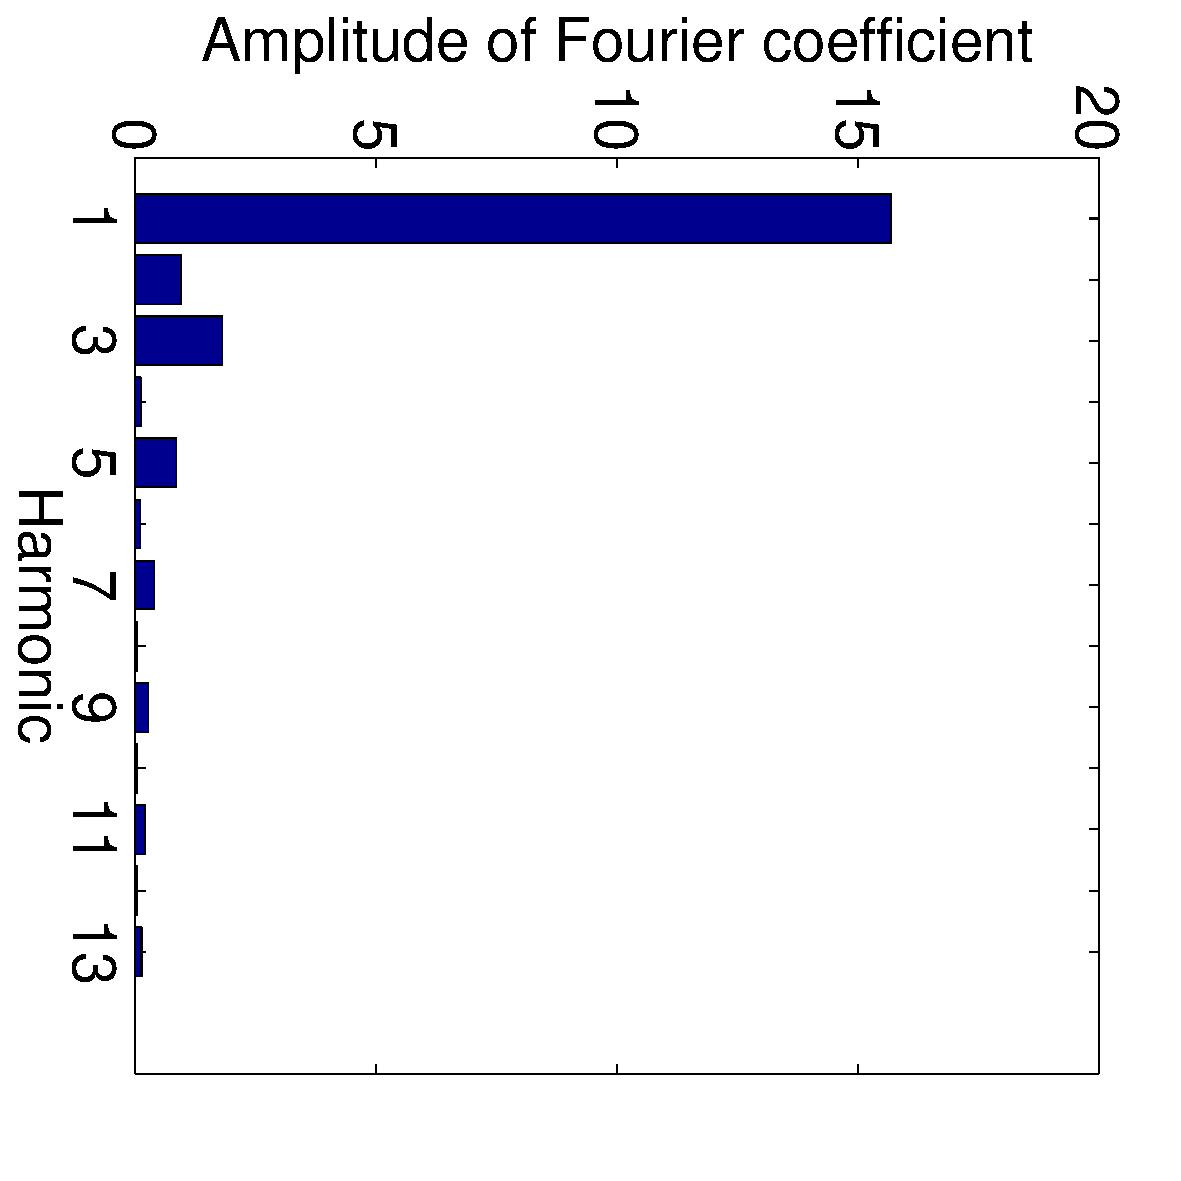
\includegraphics[width=0.33\textwidth,angle=90]{figs/refrigeratorTransientFFT.pdf} \hspace{1em}&
    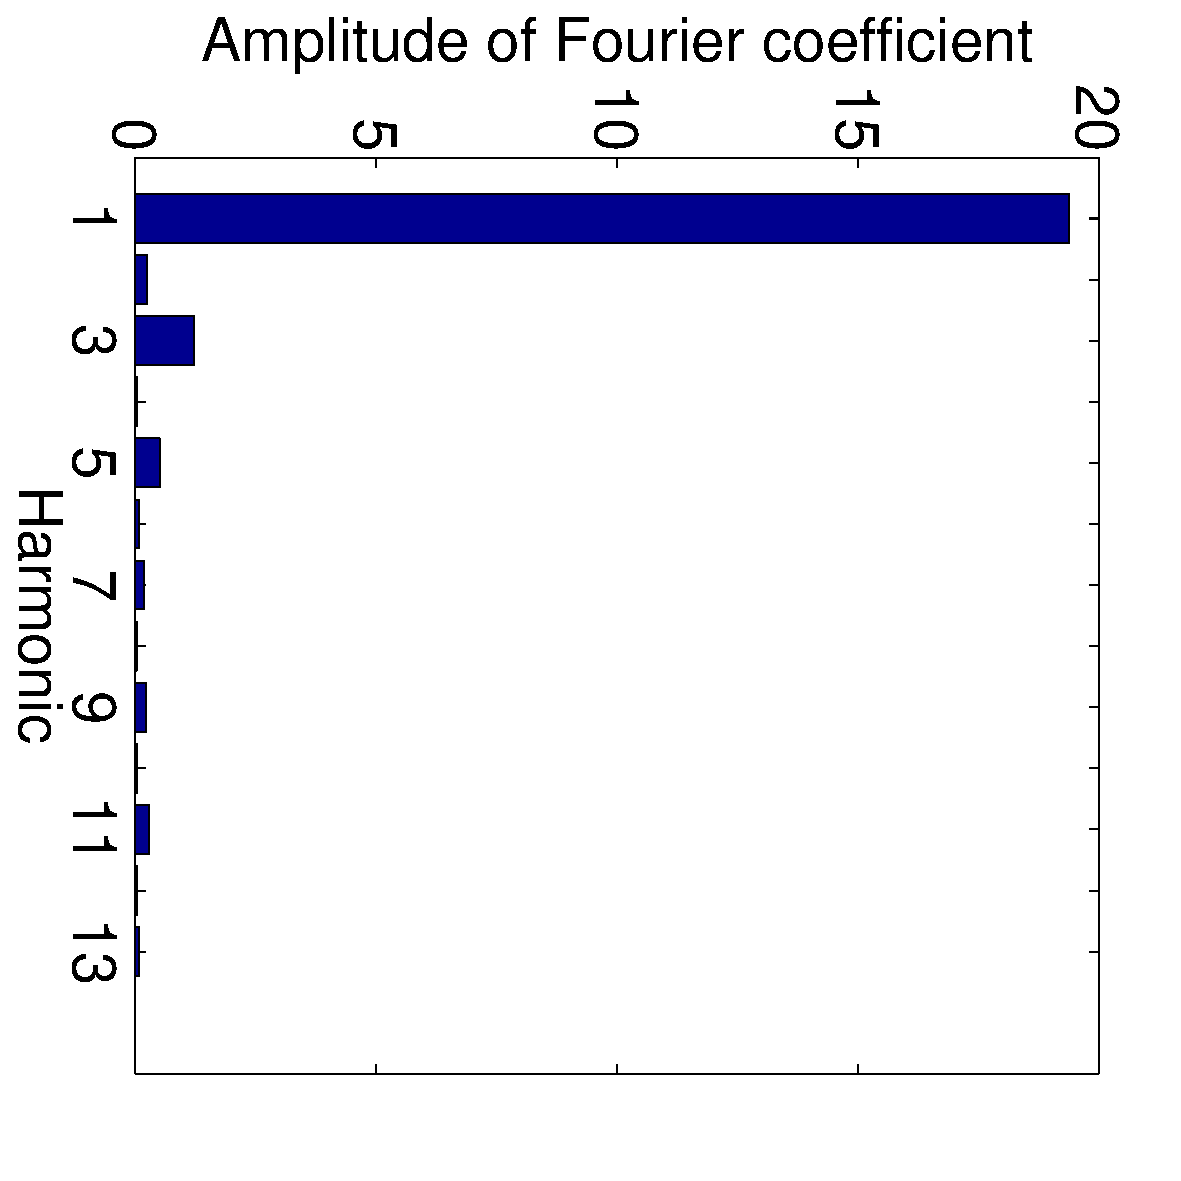
\includegraphics[width=0.33\textwidth,angle=90]{figs/airCompressorTransientFFT.pdf} \hspace{1em}&
    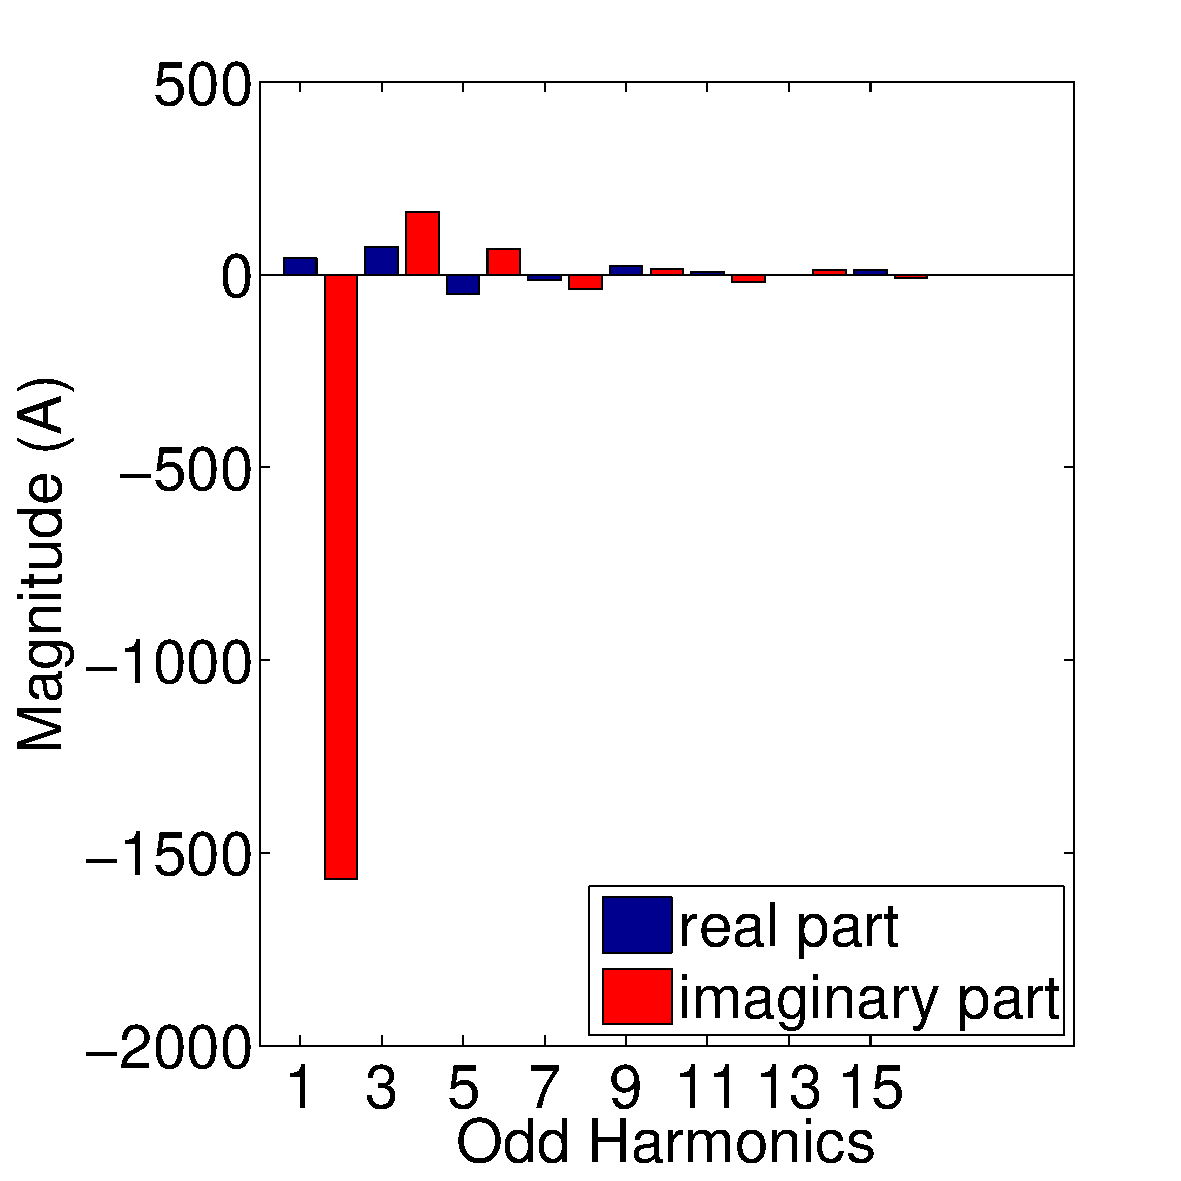
\includegraphics[width=0.33\textwidth]{figs/realImagHarmonicsRefrigerator.pdf} \tabularnewline
    (a) & (b) & (c) \tabularnewline
    \end{tabular}
    }
	\caption{Harmonics Feature of (a) a refrigerator and (b) an air compressor (c) real and imaginary part of odd number of harmonics of a refrigerator. }
	\label{fig_harmonicsFeature}
\end{figure*}
